\setcounter{figure}{0}
\setcounter{table}{0}
\setcounter{lstlisting}{0}

\chapter{Performance Evaluation}
\label{sec:performance_evaluation}
\minitoc

This chapter will describe some tests performed at the 
University of Hertfordshire (Hatfield, UK), along with 
their results. 
\\
The algorithm presented in \ref{concr:iimageselector:sweep_metric_algorithm}
(named \textit{SweepMetricAlgorithm}) was used as the image
selection algorithm. Several tests 
have been carried out, each time changing the passed parameters
(see \ref{concr:iimageselector:sweep_metric_class}).
\\
The test target is to underline the main differences 
occurring when one or more parameters change their values, 
within defined ranges. After asking users their options 
and perceptions about teleguiding the robot with an 
exocentric vision system, we could at the end identify 
the advantages and the disadvantages correlated with 
different sets of initial parameters.
\\
Since tests have been carried out using saved logs 
(see section \ref{concr:idatalogic:datalogiclogsimulator}),
users were not 
able to actually command the robot, but simply 
to request the application to go one step
further and, hence, just see the robot moving along 
the trajectory it performed during a recorded 
session.
\\
Be advised that, due to the low number of testers, 
the obtained results have not statical validity.
On the other hand, they were useful to identify 
a possible future improvement of the algorithm,
built later with \textit{Another Sweep Metric Algorithm} 
(see section \ref{concr:iimageselector:another_sweep_metric_algorithm}).

\clearpage
\subsection{Parameters}
\label{performance_evaluation:parameters}

Testing the `sweep metric algorithm' (see chapter
\ref{concr:iimageselector:sweep_metric_algorithm}) means to define
the parameters hold by the \texttt{SweepMetricCalc}
objects. All these parameters are 
to be passed to the class constructor, whose signature
is the following:

\begin{lstlisting}[caption={\texttt{SweepMetricCalc} class declaration}, label={code:sweepmetriccalc}, frame=trBL]
SweepMetricCalc::SweepMetricCalc( float sweep_angle,
				  float angle_offset,
				  float mu_distance,
				  float sigma_distance,
				  float mu_angle,
				  float sigma_angle );				  
\end{lstlisting}


With six parameters it is tricky to evaluate how changing
a single one affects on all the others. For this
reason we decided to fix same values when testing.
\\
To begin with, \texttt{sweep\_angle} has been considered a
fixed parameter during the tests. We set it to 45 degrees,
because greater values do not seem (in previous tests) to get
any advantages. On the other hand, value less than 45
degrees would not include enough images to teleguide the robot
properly.
\\
\texttt{angle\_offset} is another fixed parameter, set to 40
degrees. Exceeding this value, we risk not to include
the robot within the camera field of view, when camera and robot
present an orientation offset greater than 40 degrees.
Hence, all those images whose orientation exceeds 40 degrees
cannot compete to be the background image, 
and have to be excluded.
\\
The standard deviations \texttt{sigma\_distance} and
\texttt{sigma\_angle} belong to the set of
fixed values too. Changing the standard deviation in a Gaussian
function means only to increase or decrease its higher
point, without affecting other Gaussian properties. Because later
on it will be selected the greatest value among
all the returned ones, without any absolute reference, we do not
care about the standard deviations value.
\texttt{sigma\_distance} and \texttt{sigma\_angle} are set
with a default positive amount.
\\
In terms of Gaussian function, the \texttt{mu\_angle} represent
the mean value and, at the same time, the point where
the Gaussian function is centred. By computing the function with
\texttt{mu\_angle} in input, it will return the possible
maximum value. We remember that this function is used to calculate
a score, which has to be as greater as the difference
between the robot and image orientations are equal. Because the
function input is the difference between the two angles, it
follows that the returned value must be maximum when the input is
zero, decreasing when the input moves away from zero.
\texttt{mu\_angle} is therefore a fixed parameter, set to zero.
\\
At last, the \texttt{mu\_distance} is the unique variable parameter.
All the general consideration made before for the 
\texttt{mu\_angle} remain still valid, but this time we want to
obtain the maximum score when the difference between
robot and image position is equal to a determinant positive value,
decreasing when the difference moves away from it.
\\
If we choose a \texttt{mu\_distance} close to zero, the selected
background image will be near to the robot actual position.
The robot will be drawn only partially and the exocentric vision
will be similar to the egocentric. The more
\texttt{mu\_distance} moves away from zero (with a positive value),
the more the application will tend to draw
(when possible) all the robot to provide a full exocentric control
vision, because far image will gain an higher score.

\clearpage
\section{Test preparation}
\label{performance_evaluation:testpreparation}

The target of such tests was to verify \Item{i} if, using 
an exocentric vision system provided with such an algorithm, 
users are able to perceive the trajectory actually 
performed by the robot, \Item{ii} how much disturbing are 
sudden point-of-view changes for users, \Item{iii} how 
comfortable is for them to view a robot from a 
virtual exocentric point-of-view.
\\
People involved in the tests have had no experience in 
robotics, neither they knew what a virtual exocentric 
vision system is.
\\
The testing session schedule was the following:
\begin{enumerate}
  \item testers were given a brief introduction to exocentric vision systems
  \item each tester is given three different scenarios and has to 
    complete them, unassisted
  \item for each scenario, testers have to answer the questions 
    of a questionnaire\footnote{a copy of the questionnaire is 
      reported in this document, in section \ref{questionnaire}}
\end{enumerate}

Three different recorded logs have been used, each of which featuring 
a different trajectory. Each of such session has been tested
using three different \texttt{mu\_distance} values: 5, 15 and 25.
Results are shown in next section,
\ref{performance_evaluation:tests_result}.

\clearpage
\section{Tests results}
\label{performance_evaluation:tests_result}


\subsection{Rectangle test evaluation}
\label{performance_evaluation:tests_result:rectangletest}

Figure \ref{fig:rectangletest} shows the first test trajectory:
it is a rectangle. This path has been chosen for testing since it
features long straight segments and hard turnings (more than 80
degrees).

\begin{figure}[!h]
  \begin{center}
    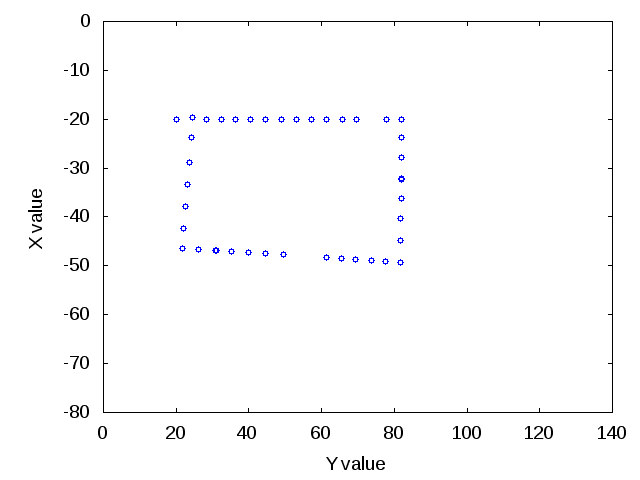
\includegraphics[width=300pt]{img/path_session_9.png}
    \caption{Rectangle trajectory test} 
    \label{fig:rectangletest}
  \end{center}
\end{figure}

\begin{figure}[!h]
  \begin{center}
    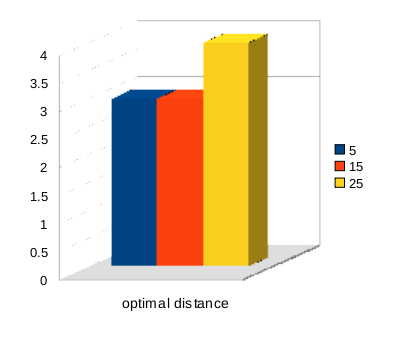
\includegraphics[width=200pt]{img/square.png}
    \caption{Users' disturbance during the rectangle test 
      by sudden change of the point-of-view over a 0/4 scale}
%%    \label{fig:rectangletest}
  \end{center}
\end{figure}

The result evidence is that most of the users figured out the
trajectory performed by the robot, even tough they perceived
sudden point of view changes during hard turnings.
\\
To sum up, they evaluated the experience positively when the
optimal distance were set to 5 or 25; not too comfortable
when set to 15.


\subsection{Ellipse test evaluation}
\label{performance_evaluation:tests_result:ellipsetest}

Figure \ref{fig:ellipsetest} shows the second test trajectory:
it is an ellipse. This path has been chosen for testing since it
features long smooth turns.

\begin{figure}[!h]
  \begin{center}
    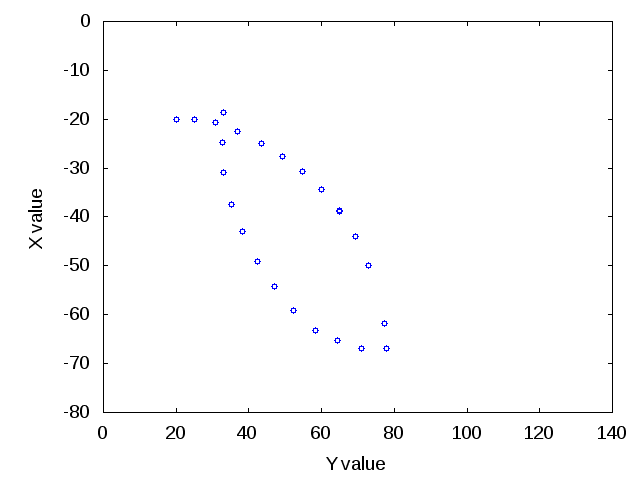
\includegraphics[width=300pt]{img/path_session_5.png}
    \caption{Ellipse trajectory test}
    \label{fig:ellipsetest}
  \end{center}
\end{figure}

\begin{figure}[!h]
  \begin{center}
    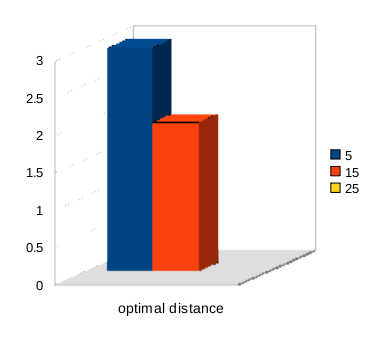
\includegraphics[width=200pt]{img/ellipse.png}
    \caption{Users' disturbance during the ellipse test 
      by sudden change of the point-of-view over a 0/4 scale}
    %%    \label{fig:rectangletest}
  \end{center}
\end{figure}
%
The result evidence is that all of the users figured out the
trajectory performed by the robot. This case allows to point out
a specify trend: the more the optimal distance is, the less users
perceive sudden point of view changes.
\\
Testers also reported they had very comfortable experience.


\subsection{Broken lines test evaluation}
\label{performance_evaluation:tests_result:zigzagtest}

Figure \ref{fig:zigzagtest} shows the third test trajectory:
it is made up of broken lines. This path has been chosen for testing
since it features straight lines and sudden hard turnings.

\begin{figure}[!h]
  \begin{center}
    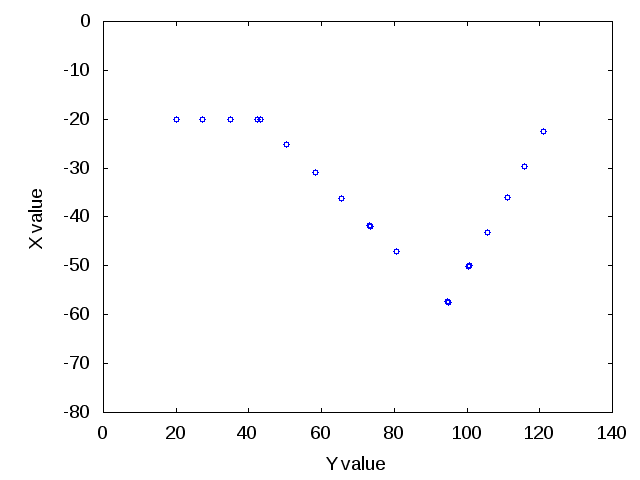
\includegraphics[width=300pt]{img/path_session_6.png}
    \caption{Broken lines trajectory test}
    \label{fig:zigzagtest}
  \end{center}
\end{figure}

\begin{figure}[!h]
  \begin{center}
    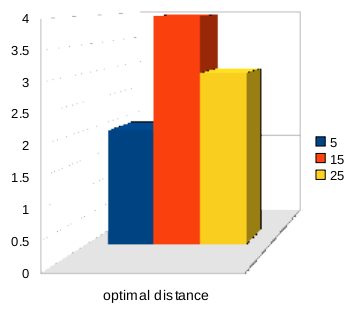
\includegraphics[width=200pt]{img/zz_results.png}
    \caption{Users' disturbance during the broken lines test 
      by sudden change of the point-of-view over a 0/4 scale}
%%    \label{fig:rectangletest}
  \end{center}
\end{figure}

The result evidence is the users did not recognise the performed path.
Moreover, it also emerged that the more the optimal distance is short,
the less are the occurrences of sudden point of view changes.
\\
For the reasons above, testers reported a not very comfortable experience.

\clearpage
\subsection{Final considerations}
\label{performance_evaluation:tests_result:finalconsiderations}
According to us, two chief conclusion can be drawn.
\\
The former is that when the robot moves along straight lines
the optimal distance should be set to higher values, in order
to show the entire robot model and, hence, to give a \textit{fully}
exocentric vision.
\\
The latter one regards turnings. When robot performs hard turnings
the \textit{sweep metric algorithm} often selects the egocentric
point of view: changing from an exocentric to an egocentric vision
causes disturbance to users.
\\
To overcome this deficiency an evolution of the \textit{sweep metric
algorithm} was afterwards developed. It is named \textit{another sweep
metric algorithm} (proving the authors' lack of imagination), and
exposed in sections 
\ref{concr:iimageselector:another_sweep_metric_algorithm} and
\ref{concr:iimageselector:another_sweep_metric_class}.
\\
Even though the new algorithm has never been tested with users, its
benefits are immediately evident, in particular if the robot moves
along a `square' path, where long straight distances are interspersed
with strict turns (angles greater than 45 degrees).

